\begin{center}
    {\LARGE \textbf{2019有机化学}} \\[2ex]
    {\large 时量180分钟 \quad 满分150分}
\end{center}

\vspace{0.5cm}
\noindent\textbf{注意事项:}
\begin{enumerate}[label=\arabic*., parsep=0pt, itemsep=0pt]
    \item 答题前,考生先将自己的姓名、学号、考场号、座位号填写在答题卡上,将条形码准确粘贴在考生信息条形码粘贴区。
    \item 考试结束后,将本试卷与答题纸一并收回。
    \item 回答各个问题时,将答案写在答题纸上,写在本试卷上无效。
\end{enumerate}

\vspace{0.5cm}
\noindent\textbf{一、选择题（15 pts.）}

\begin{enumerate}[label=\arabic*., itemsep=1.5ex]
    \item 不具有芳香性的化合物是
    
    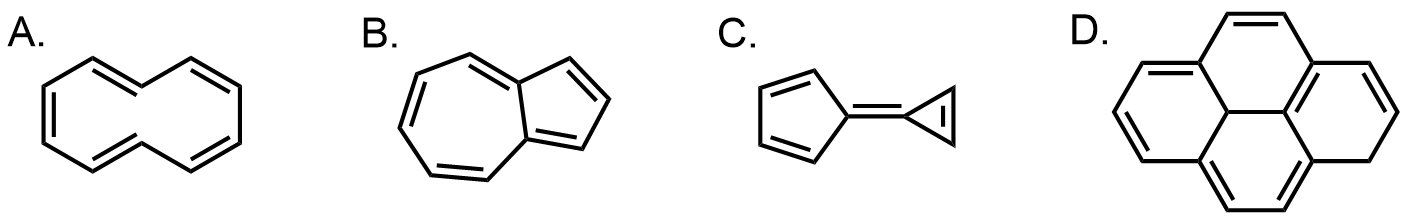
\includegraphics[scale=0.38, valign=c]{./Figure/2019/2019_4_1.png}
    \item 以下最稳定的极限式是
    
    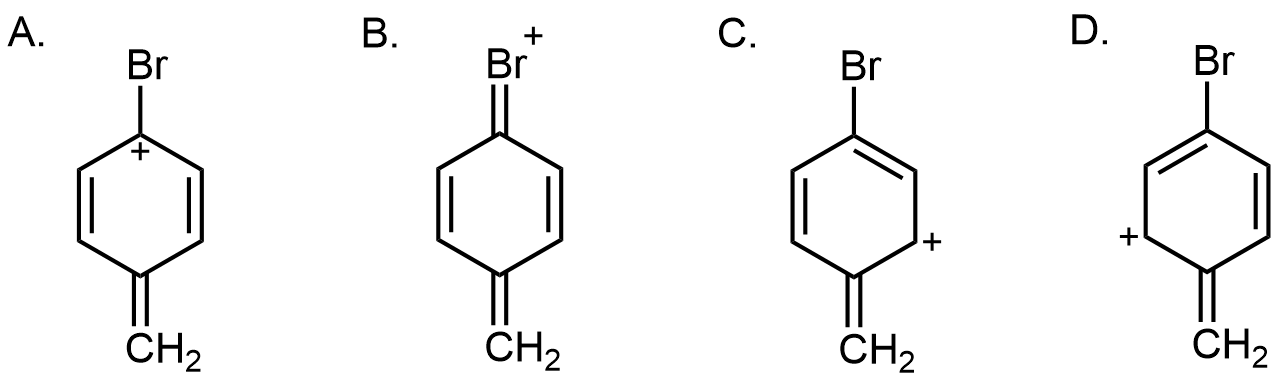
\includegraphics[scale=0.38, valign=c]{./Figure/2019/2019_4_2.png}
    \item 不能用于从水相萃取有机物的溶剂是
    \begin{tasks}(4)
        \task 四氯化碳
        \task 丙酮
        \task 环己烷
        \task 乙醚
    \end{tasks}
    \item 与1,3-丁二烯发生Diels-Alder反应时，反应速率最快的是
    
    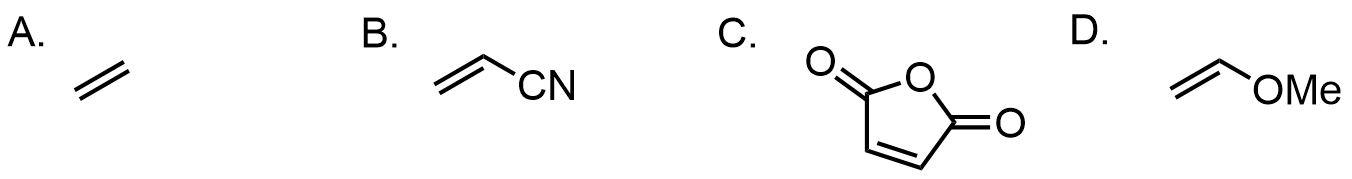
\includegraphics[scale=0.38, valign=c]{./Figure/2019/2019_4_4.png} 
    \item 可用于分离苯甲酸和苯甲醇的方法是
    \begin{tasks}(4)
        \task 重结晶
        \task 萃取
        \task 减压蒸馏
        \task 水蒸气蒸馏
    \end{tasks}
    \item 在以下哪个溶剂中\ce{CH3OH}的亲核性最强
    \begin{tasks}(4)
        \task DMSO
        \task 水
        \task TFA
        \task EtOH
    \end{tasks}
    \item 具有手性的分子是
    
    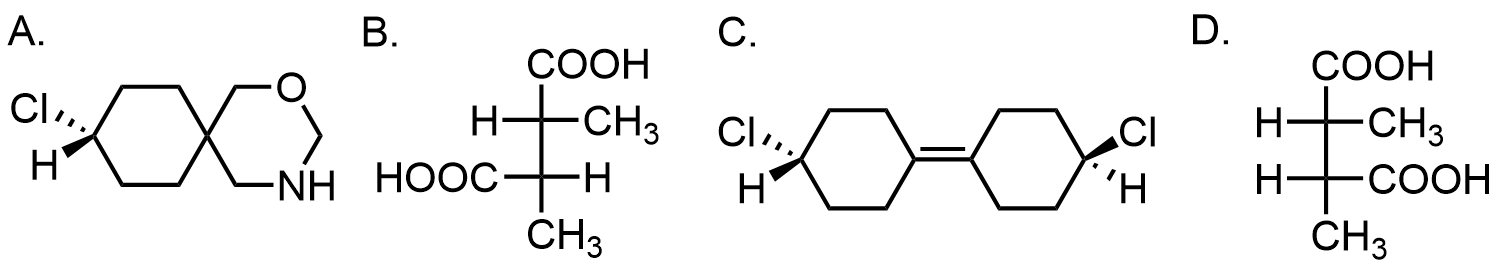
\includegraphics[scale=0.38, valign=c]{./Figure/2019/2019_4_7.png}
    \item 酸性最强的化合物是
    
    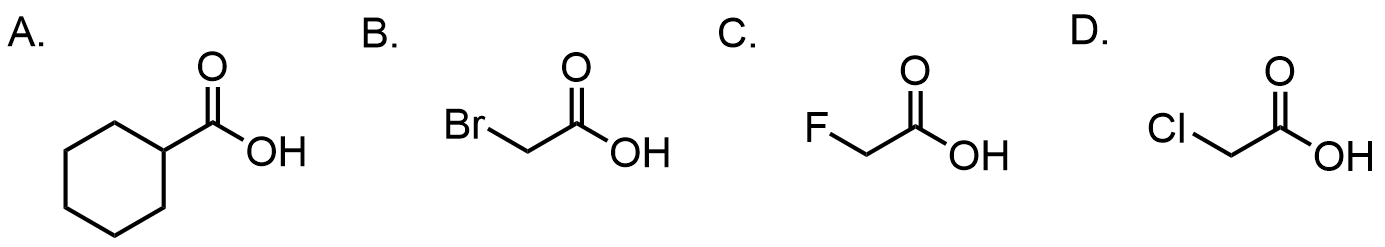
\includegraphics[scale=0.38, valign=c]{./Figure/2019/2019_4_8.png}
    \item 难以发生Friedel-Crafts酰基化反应的化合物是
    
    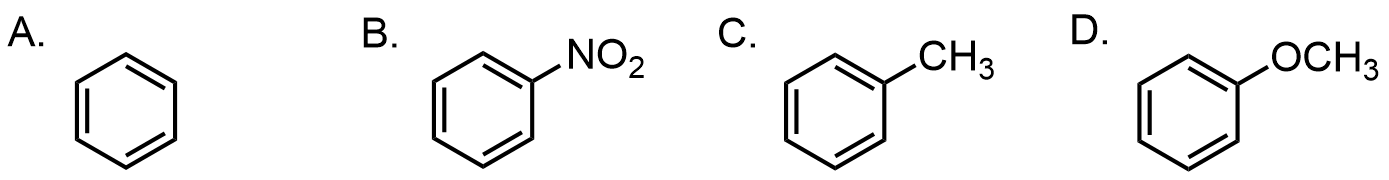
\includegraphics[scale=0.38, valign=c]{./Figure/2019/2019_4_9.png}
    \item 与\ce{AgNO3}反应最快的化合物是
    
    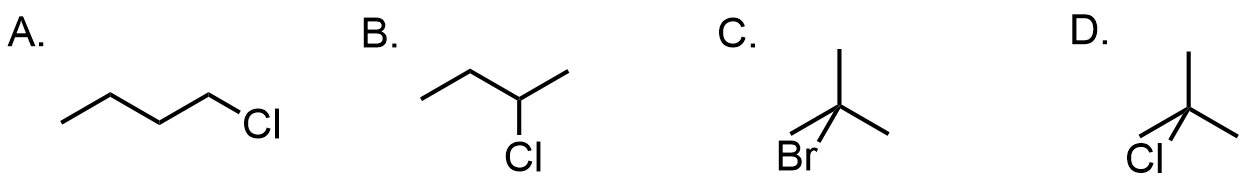
\includegraphics[scale=0.38, valign=c]{./Figure/2019/2019_4_10.png}
    \item 不能与HCN反应的化合物是
    \begin{tasks}(4)
        \task 葡萄糖
        \task 苯乙酮
        \task 糠醛
        \task 2-戊酮
    \end{tasks}
    \item 最稳定的碳正离子是
    
    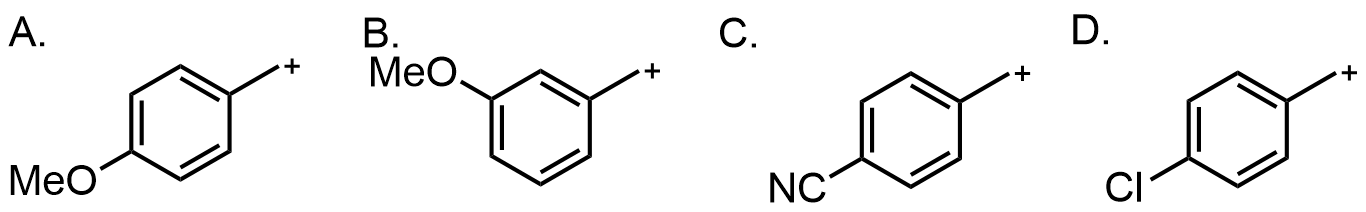
\includegraphics[scale=0.38, valign=c]{./Figure/2019/2019_4_12.png}
    \item 如下分子中碱性最强的N是
    
    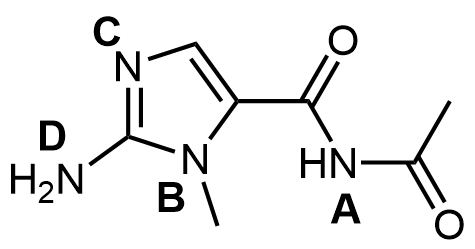
\includegraphics[scale=0.38, valign=c]{./Figure/2019/2019_4_13.png}
    \item 如下分子中手性碳原子的绝对构型是

    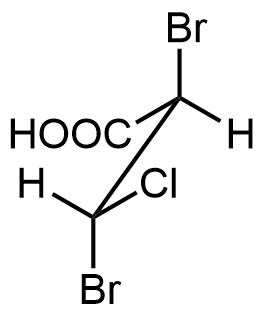
\includegraphics[scale=0.38, valign=c]{./Figure/2019/2019_4_14.png}
    \begin{tasks}(4)
        \task 2R, 3R
        \task 2S, 3S
        \task 2R, 3S
        \task 2S, 3R
    \end{tasks}
    \item 与Lucas试剂反应，体系立刻变浑浊的是
    \begin{tasks}(4)
        \task 正丁醇
        \task 乙醇
        \task 丙烯醇
        \task 环戊醇
    \end{tasks}
\end{enumerate}

\vspace{0.5cm}
\noindent\textbf{二、完成反应(50 pts.)}

\begin{enumerate}[label=\arabic*., itemsep=3ex]
    \item 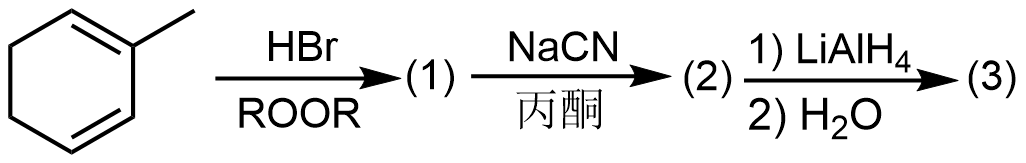
\includegraphics[scale=0.3, valign=c]{./Figure/2019/2019_1_1.png} 
    \item 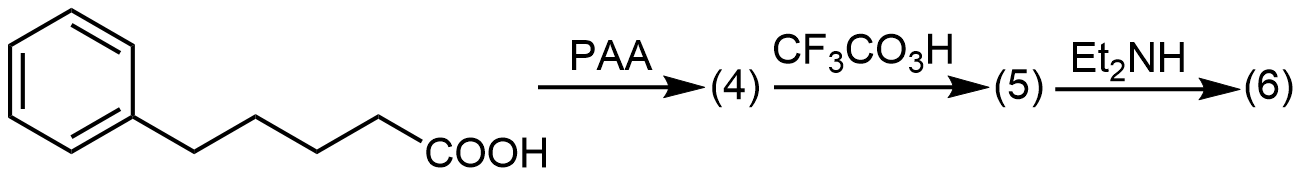
\includegraphics[scale=0.3, valign=c]{./Figure/2019/2019_1_2.png}
    \item 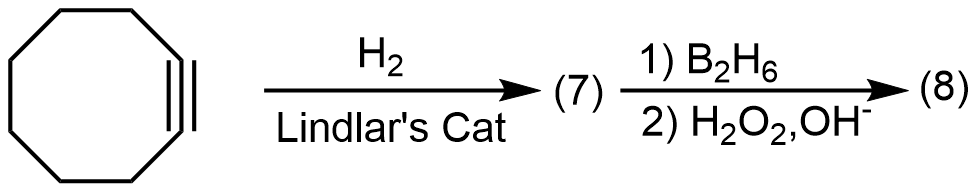
\includegraphics[scale=0.3, valign=c]{./Figure/2019/2019_1_3.png}
    \item 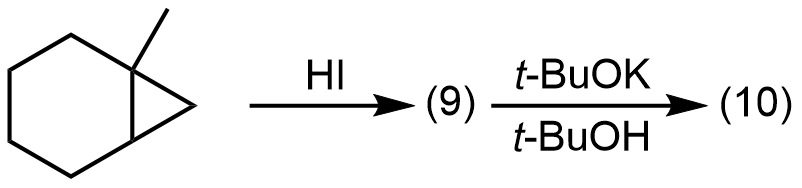
\includegraphics[scale=0.3, valign=c]{./Figure/2019/2019_1_4.png}
    \item 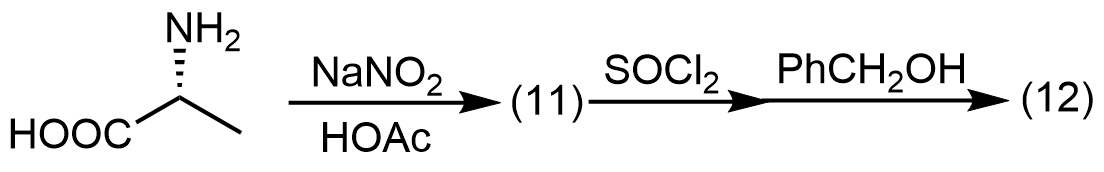
\includegraphics[scale=0.3, valign=c]{./Figure/2019/2019_1_5.png}
    \item 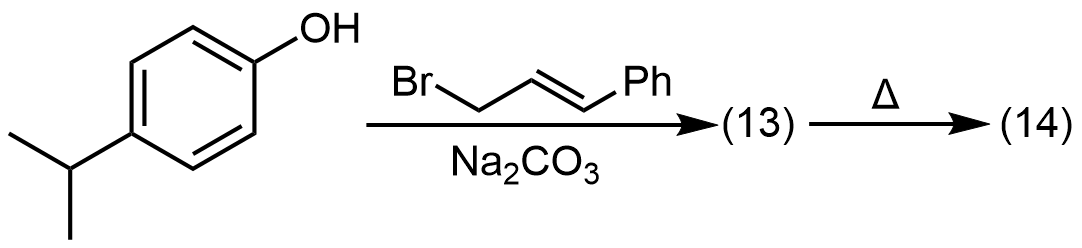
\includegraphics[scale=0.3, valign=c]{./Figure/2019/2019_1_6.png}
    \item 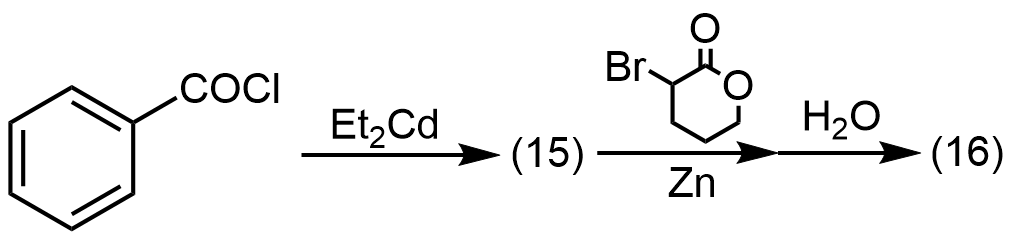
\includegraphics[scale=0.3, valign=c]{./Figure/2019/2019_1_7.png}
    \item 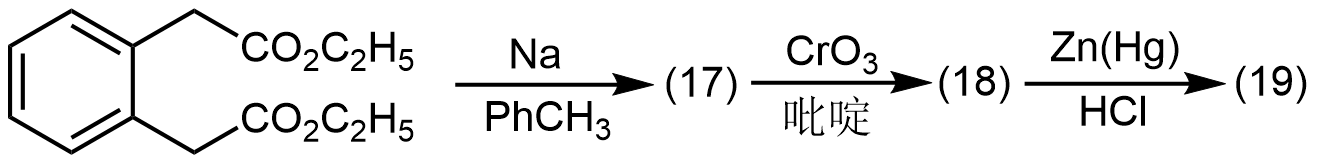
\includegraphics[scale=0.3, valign=c]{./Figure/2019/2019_1_8.png}
    \item 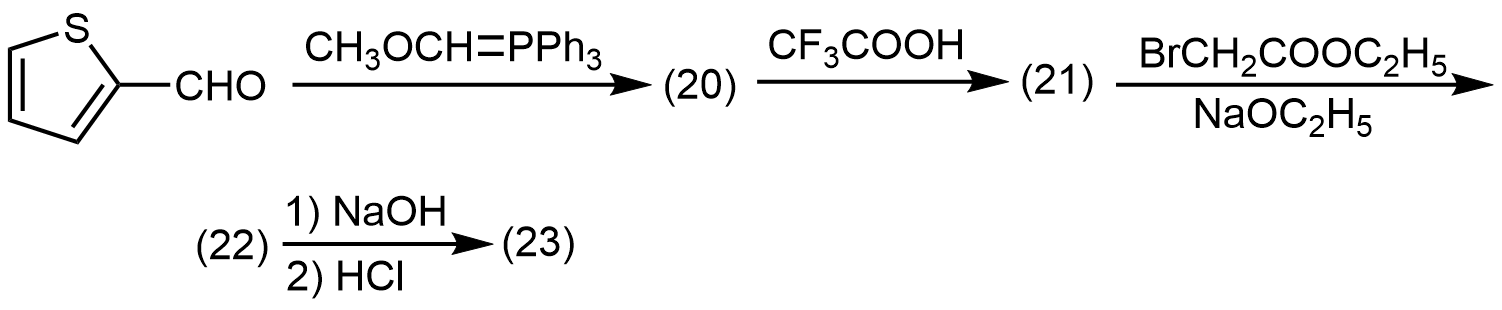
\includegraphics[scale=0.3, valign=c]{./Figure/2019/2019_1_9.png}
    \item 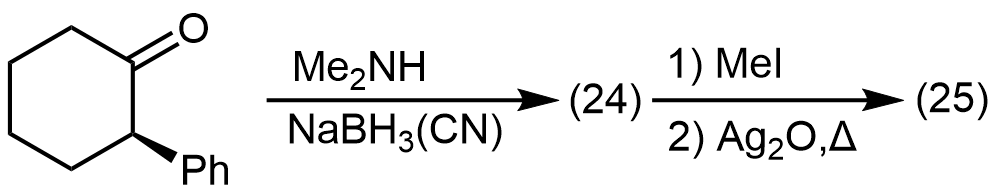
\includegraphics[scale=0.3, valign=c]{./Figure/2019/2019_1_10.png}

\end{enumerate}

\vspace{0.5cm}
\noindent\textbf{三、机理题(28 pts.)}

\begin{enumerate}[label=\arabic*., start=1, itemsep=1.5ex]
    \item 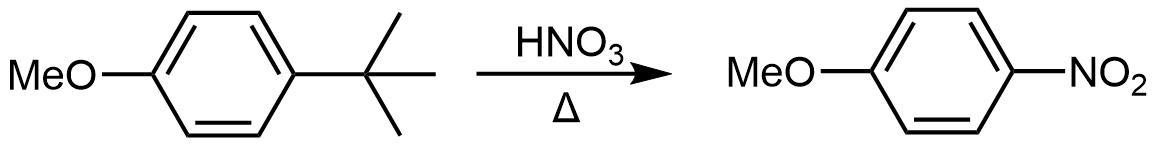
\includegraphics[scale=0.3, valign=c]{./Figure/2019/2019_2_1.png}
    \item 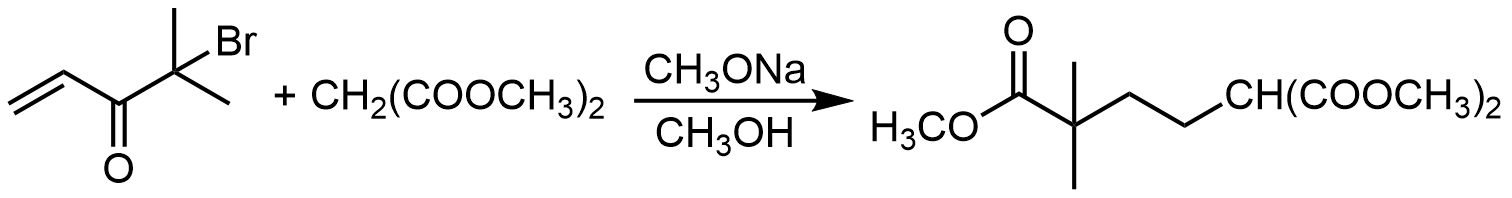
\includegraphics[scale=0.3, valign=c]{./Figure/2019/2019_2_2.png}
    \item 写出反应的主要产物，并提出合理的分步机理
    
    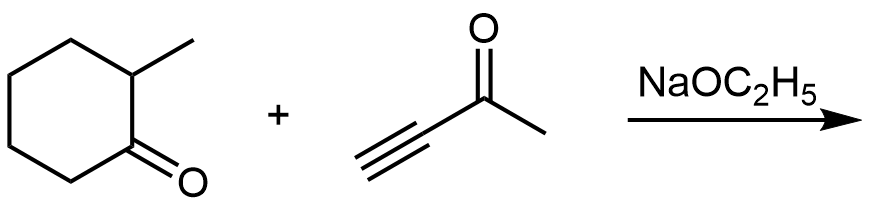
\includegraphics[scale=0.3, valign=c]{./Figure/2019/2019_2_3.png}
    \item 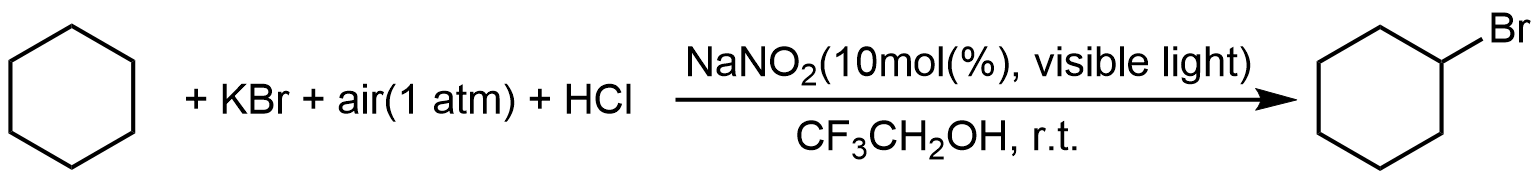
\includegraphics[scale=0.3, valign=c]{./Figure/2019/2019_2_4.png}
\end{enumerate}

\newpage

\vspace{0.5cm}
\noindent\textbf{四、合成题(42 pts.)}

\begin{enumerate}[label=\arabic*., start=1, itemsep=1.5ex]

    \begin{figure}[htbp]
        \centering
        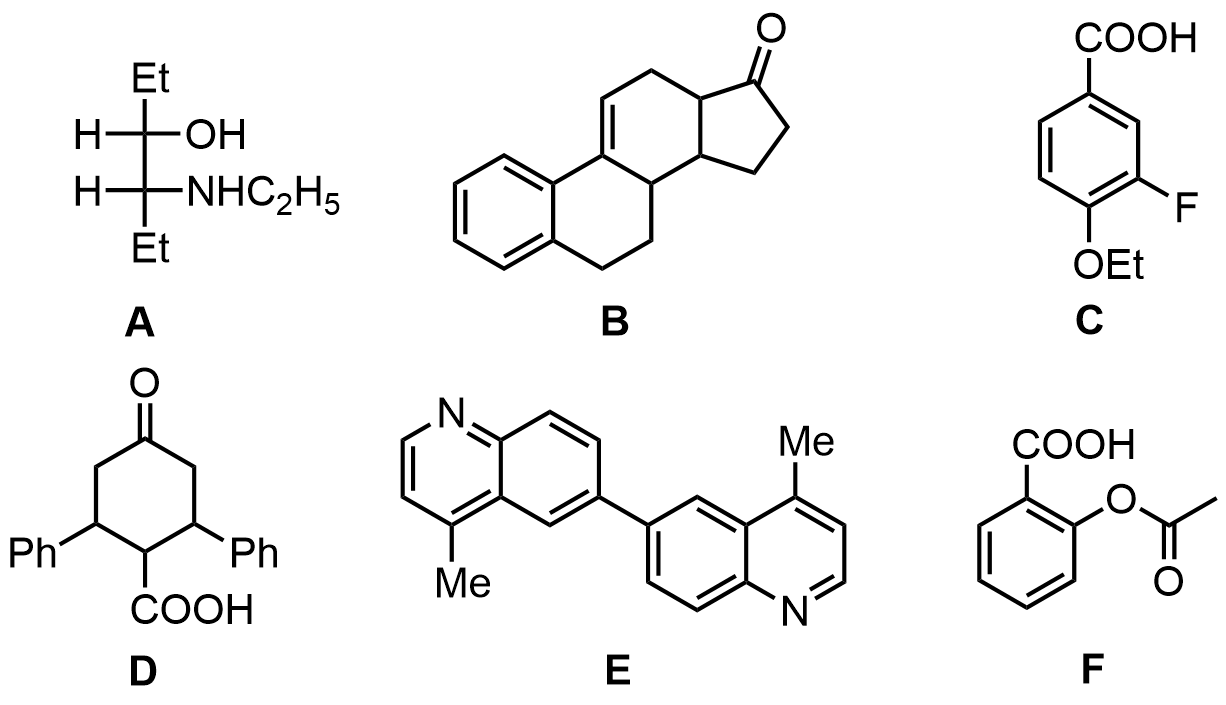
\includegraphics[scale=0.38]{./Figure/2019/2019_3.png}
    \end{figure}
    \item 以小于等于2个碳的有机物合成\textbf{A}
    \item 以苯、小于等于5个碳的有机物合成\textbf{B}
    \item 以甲苯为主要原料合成\textbf{C}
    \item 以苯、小于等于4个碳的有机物合成\textbf{D}
    \item 以苯、小于等于3个碳的有机物合成\textbf{E}
    \item 以苯或甲苯为主要原料合成阿司匹林\textbf{F}
\end{enumerate}

\vspace{0.5cm}
\noindent\textbf{五、实验题 略}